\documentclass{article}
\usepackage[utf8]{inputenc}
\usepackage[brazil]{babel}
\usepackage{hyperref}
\usepackage{indentfirst}
\usepackage{xcolor}
\usepackage{amsfonts}
\usepackage{amsmath}
\usepackage{amssymb}
\usepackage{amsthm}
\usepackage{graphicx}
\usepackage{minted}
\usepackage{xurl}
\usepackage{float}
\usepackage{csquotes}
\usepackage[a4paper, left=4cm, right=4cm]{geometry}
\usepackage{colortbl}
\usepackage[backend=biber,style=numeric]{biblatex}
\addbibresource{referencias.bib}

%Formata hrefs
\hypersetup{
    colorlinks=true,
    linkcolor=black,
    filecolor=magenta,      
    urlcolor=blue,
    pdftitle={Trabalho},
    pdfpagemode=FullScreen,
    }

\title{Relatório - Field Projecto desenvolvimento com a Cartesius Capital}
\author{Daniel Miranda, Kauan Mariani, Pedro Coterli, Leonardo Alexandre}
\date{\today}

%%%%%%%%%%%%%%%%%%%%%%%%%%%%%%%%%%%%%%%%%%%%%%%%%

\begin{document}

%Cria a capa do trabalho
\begin{titlepage}
    \begin{center}            
        \Huge
        \textbf{Field Project - Cartesius Capital}
            
        \vspace{0.5cm}
        \LARGE
        %P* - A*
            
        \vspace{3.0cm}

        \textbf{Daniel de Miranda Almeida}\\
        \textbf{Kauan Mariani Ferreira}\\
        \textbf{Pedro Henrique Coterli}\\
        \textbf{Leonardo Alexandre da Silva Ferreira}

        \vspace{3.0cm}
            
            
        Relatório apresentando trabalho desenvolvido durante Projeto de Campo ministrado pelo Dr. Walter Wagner Carvalho Sande em parceria com a Cartesius Capital
            
        \vspace{1.0cm}
            
        
\includegraphics[width=0.4\textwidth]{imagens/Logo FGV.png}
            
        \Large
        Escola de Matemática Aplicada\\
        Fundação Getulio Vargas\\
        Rio de Janeiro, RJ - Brasil\\
        \today
            
    \end{center}
\end{titlepage}
\newpage

%Cria Sumário automaticamente
\tableofcontents
\newpage

\section{Introdução}

O mercado financeiro é caracterizado por sua alta complexidade e dinamicidade, onde a identificação de tendências desempenha um papel crucial na tomada de decisões estratégicas. Uma das abordagens mais populares para análise de dados financeiros é o uso de estratégias de \textit{trend following}. Esse método busca capturar movimentos persistentes no preço de ativos, aproveitando as tendências predominantes, sejam de alta ou de baixa. A premissa subjacente é que, uma vez estabelecida, uma tendência tende a continuar por um período, permitindo que investidores ou sistemas automatizados realizem operações com base nesse padrão.

Tradicionalmente, o \textit{trend following} tem sido implementado por meio de indicadores técnicos, como médias móveis e o \textit{MACD} (\textit{Moving Average Convergence Divergence}). Esses indicadores analisam dados históricos de preço e volume para gerar sinais de compra e venda. No entanto, isoladamente, cada indicador possui limitações e está sujeito a falsos positivos, especialmente em mercados voláteis ou com mudanças rápidas de regime.

Com o avanço da tecnologia, o campo de \textit{machine learning} emergiu como uma solução poderosa para superar essas limitações. Modelos de aprendizado de máquina podem processar grandes volumes de dados e identificar padrões complexos que seriam difíceis de detectar manualmente. Ao integrar múltiplos indicadores técnicos e variáveis de mercado, esses modelos conseguem extrair insights mais robustos e tomar decisões mais informadas. Além disso, técnicas como \textit{ensemble learning} e redes neurais permitem combinar os pontos fortes de diferentes abordagens, resultando em previsões mais precisas e confiáveis.

Este trabalho foi desenvolvido em parceria entre a Escola de Matemática Aplicada da Fundação Getulio Vargas (EMAp-FGV) e a Cartesius Capital, uma empresa que se posiciona como uma \textit{fundtech}, inovando na gestão de fundos multimercado com o uso de sistemas de inteligência artificial preditiva. Diferentemente de gestoras tradicionais, a Cartesius Capital combina métodos quantitativos avançados, tecnologia de ponta e análise situacional para identificar oportunidades de investimento em ativos de elevada liquidez nos mercados financeiros globais.

O projeto é um \textit{side project} da Cartesius Capital, com a colaboração de alunos do quarto período da graduação em Ciência de Dados e Inteligência Artificial da EMAp-FGV. O objetivo central é criar um modelo de \textit{trend following} para ativo com poucos dados e assim capitalizar oportunidades de mercado com maior frequência e eficácia. Por meio da integração de uma vasta gama de indicadores técnicos e algoritmos de aprendizado supervisionado, buscamos construir um sistema de suporte à decisão que não apenas detecte tendências, mas também se adapte às mudanças nas condições de mercado, mantendo uma performance consistente ao longo do tempo.

Segue o link do repositório no qual o projeto foi desenvolvido: \url{https://github.com/kauanmaf/field_project_cartesius}.


\section{Rotulador}

O método escolhido para rotulagem dos dados é o método de barreira tripla \cite{Prado}, que funciona da seguinte maneira: para um horizonte de tempo $h$ são definidas três barras: duas horizontais que definem os limiares \textit{profit-taking} e o \textit{stop-loss} para o retorno daquele período e uma terceira, vertical, que é atingida caso nenhuma das barras verticais seja cruzada antes do fim do horizonte de tempo $h$. Caso as barras horizontais sejam cruzadas, o algoritmo rotula aquele período como 1 (deve-se ficar comprado) se a barra superior for atingida, ou como -1 (deve-se ficar vendido). Se a barra vertical for atingida, temos uma tendência à média 0 e o dado é rotulado como 0 (ficar inerte)

\subsection{Retornos Logarítmicos}

A rotulagem é feita utilizando o retorno logarítmico dos preços, que tem a seguinte fórmula:

$$ r_t = ln \left( \frac{P_t}{P_{t - 1}} \right) $$

onde:
\begin{itemize}
    \item $r_t$ é o retorno no tempo $t$
    \item ${P_t}$ é o preço da ação no tempo $t$
    \item $P_{t - 1}$ é o preço da ação no período de tempo anterior $t - 1$
\end{itemize}

\subsubsection{Por que retornos logarítmicos?}

A escolha de retornos logarítmicos foi feita porque eles apresentam uma série de características vantajosas, dentre as quais cita-se algumas:

\begin{itemize}
    \item \textbf{Aditividade temporal (efeito composto)}: o retorno logarítmico é aditivo temporalmente, isto é, o retorno total sobre múltiplos períodos de tempo é igual à soma dos retornos logarítmicos individuais. Como dados financeiros geralmente apresentam um comportamento cumulativo ao longo do tempo, o uso de retornos logarítmicos é mais adequado, principalmente com longos intervalos temporais. \cite{Hull}
    \item \textbf{Mais estabilidade e robustez frente a grandes flutuações}: grandes flutuações em preços são mais estabilizados pela medida logaritmica de retorno. Enquanto um retorno simples pode exagerar os efeitos de grandes mudanças de preços, o retorno logarítmico dá uma perspectiva mais estável. \cite{Bouchaud}
\end{itemize}

\subsection{Limiares dinâmicos}

Os limiares de \textit{profit-taking} e \textit{stop-loss} são definidos de acordo com o Desvio Padrão Móvel Ponderado Exponencialmente (\textit{EWMSD - Expontentially Weighted Moving Standard Deviation}), que, grosso modo, calcula o desvio padrão móvel dos preços (semelhante à média móvel, mas para o desvio padrão) e os pondera de maneira exponencial, ou seja, priorizando a relevância de valores mais recentes e decaindo exponecialmente a relevância para valores mais antigos. Isso faz com que, mesmo que os preços recentes sejam os mais importantes para a compreensão da volatilidade, todo o movimento acumulado é relevante para se perceber uma tendência.

\subsubsection{Fórmula do \textit{EWMSD}}
Dada uma série de retornos $x_1, x_2, \dots, x_n$, segue-se os seguintes passos.

\begin{enumerate}
    \item Calcula-se a \textbf{Média Móvel Ponderada Exponeniclamente (\textit{Exponentially Weighted Moving Average - EWMA})}: $$EWMA_t = \lambda \cdot x_t + (1 - \lambda) \cdot EWMA_{t - 1}$$ onde:

    \begin{itemize}
        \item $\lambda$ é o fator de decaimento que determina quão rapidamente o peso para os dados passados decai.
        \item $x_t$ é o valor no tempo $t$
        \item $EWMA_{t - 1}$ é a \textit{EWMA} do passo anterior
    \end{itemize}
    
    \item Calcula-se a \textbf{Variância Ponderada Exponeniclamente (\textit{Exponentially Weighted Moving Variance - EWMV})}: $$EWMV_t = \lambda \cdot (x_t - EWMA_t)^2 + (1 - \lambda) \cdot EWMV_{t - 1}$$.
    
    \item E por fim a \textbf{\textit{EWMSD}}: $$EWMSD_t = \sqrt{EWMV_t}$$
\end{enumerate}

\subsubsection{Por que \textit{EWMSD}?}

\cite{Knight} O uso da \textit{EWMSD} é interessante por alguns motivos:

\begin{itemize}
    \item \textbf{Efeito de suavização}: Como o cálculo também dá importância para valores passados de volatilidade, há uma maior robustez contra ruídos de valores no curto prazo, o que é essencial para o bom treinamento de modelo de aprendizado de máquina. Contudo, como o peso dado aos valores ao longo do tempo decai exponencialmente, a \textit{EWMSD} ainda é bastante sensível a dados recentes, de forma que  reage em tempo hábil a mudanças de tendências.
    
    \item \textbf{Identificação de Acúmulos de Volatilidade}: a volatilidade em mercados tende a se acumular sobre períodos de tempo, com períodos de alta volatilidade tendendo a ser seguidos por períodos de mais alta volatilidade. A estatística ajuda a modelar esse comportamento se adaptando a volatilidades recentes enquanto recursivamente acumula volatilidades passadas.
\end{itemize}

\newpage

\section{Modelos de Machine Learning}

Anteriormente, extraiu-se uma lista de indicadores dos dados referentes aos ativos, que foram normalizados. Após essa extração, realizou-se uma rotulagem dos dados. 

Dados esses passos, pode-se realizar o treinamento dos dados com os seus rótulos. Assim, três modelos de machine learning foram elaborados.

\subsection{Rede Neural}

Uma rede neural é um modelo que toma decisões semelhantes ao cérebro humano, pois utiliza processos que imitam o modo como os neurônios trabalham juntos para realizar conclusões.

Toda rede neural é composta por camadas de nós (neurônios artificiais): uma camada de entrada, uma ou mais camadas ocultas e uma camada de saída.

As redes neurais dependem de dados de treinamento para aprender e melhorar sua precisão ao longo do tempo. Uma vez ajustadas para precisão, tornam-se ferramentas poderosas para a classificação e o agrupamento dos dados com alta velocidade. 

\subsection{Random Forest}

O Random Forest é um algoritmo de machine learning que usa vários subconjuntos de dados de treinamento para construir uma série de árvores de decisão. Cada árvore é treinada de forma independente e focada em diferentes características dos dados, o que aumenta a diversidade entre as árvores.

Esse modelo tem o objetivo de realizar previsões mais robustas e precisas ao combinar os resultados de todas as árvores. As previsões finais são realizadas por votação majoritária (para classificação) ou pela média (para regressão).

\subsection{Gradient Boosting}

O Gradient Boosting é um algoritmo de aprendizado de máquina que produz um modelo de previsão na forma de um conjunto de modelos de previsão fracos de modo sequencial, o que permite a otimização de uma função de perda diferenciável arbitrária.

Aos ajustes de cada modelo fraco, multiplica-se um valor chamado de taxa de aprendizagem, que tem como objetivo determinar o impacto de cada árvore no modelo final. Quanto menor o valor, menor a contribuição de cada árvore.

Em suma, o propósito do algoritmo é criar uma corrente de modelos fracos, em que cada um tem como objetivo minimizar o erro do modelo anterior por meio de uma função de perda.

\subsection{Modelo de Treinamento}

Após realizar testes preliminares com uma versão inicial do modelo e utilizando algumas \textit{features} selecionadas, observamos que o \textit{Random Forest} apresentou o melhor desempenho em relação aos outros algoritmos avaliados. Além de alcançar resultados comparáveis aos modelos mais complexos, o \textit{Random Forest} destacou-se por sua eficiência computacional, exigindo baixo custo de processamento e oferecendo rápida execução. 

Considerando essas vantagens, optamos por concentrar os esforços no desenvolvimento e teste de modelos de \textit{trend following} utilizando exclusivamente o \textit{Random Forest} como algoritmo de \textit{machine learning}. Essa abordagem permitiu uma maior agilidade nos experimentos, sem comprometer a qualidade dos resultados obtidos.

\newpage

\section{Indicadores}
A proposta do modelo de \textit{machine learning} baseou-se no uso de indicadores de \textit{trend following} amplamente conhecidos, com o objetivo de identificar padrões nos dados financeiros. A inspiração inicial veio do livro \textit{Mastering Financial Pattern Recognition: Finding and Back-Testing Candlestick Patterns with Python} \cite{Kaabar}, que apresenta diversos indicadores para sinalizar oportunidades de compra e venda. No entanto, os indicadores sugeridos no livro geravam um número limitado de operações, resultando em poucos \textit{trades} por ano. Esse comportamento não atendia ao nosso objetivo de desenvolver um modelo que realizasse operações com maior frequência.

Para contornar essa limitação, utilizamos a biblioteca \texttt{ta} (\textit{Technical Analysis}) em Python, que disponibiliza uma ampla gama de indicadores de \textit{trend following} implementados. O objetivo foi combinar diversos indicadores amplamente utilizados no mercado financeiro e disponíveis nessa biblioteca, de modo a criar um conjunto abrangente de variáveis preditivas. A premissa central era que cada indicador, isoladamente, poderia apresentar um desempenho modesto; contudo, ao integrá-los por meio de \textit{machine learning}, esperávamos construir um modelo mais robusto, capaz de superar a performance individual de cada indicador. 


Os indicadores foram agrupados em três principais categorias: \textbf{Trend Indicators}, \textbf{Oscillators} e \textbf{Volume-Based Indicator}. A seguir, detalhamos os indicadores selecionados:

\subsection{Trend Indicators}

Os \textit{Trend Indicators} são projetados para identificar a direção geral do mercado, ajudando a determinar se um ativo está em tendência de alta, baixa ou lateral.

\begin{itemize}
    \item \textbf{Moving Average Convergence Divergence (MACD):} Utilizado para identificar mudanças na força, direção e duração de uma tendência no preço.
    
    \item \textbf{Aroon Indicator:} Indica a força de uma tendência e a probabilidade de reversão.

    \item \textbf{Schaff Trend Cycle (STC):} Um oscilador baseado em ciclos, projetado para identificar tendências de maneira mais rápida que o MACD.

    \item \textbf{Ichimoku Cloud:} Uma ferramenta abrangente que identifica suporte, resistência, direção de tendência e força.

    \item \textbf{KST Oscillator:} Um oscilador baseado em múltiplos períodos de taxa de variação, útil para capturar a dinâmica da tendência.

    \item \textbf{Average Directional Index (ADX):} Mede a força de uma tendência, independentemente de sua direção.

    \item \textbf{Parabolic SAR:} Identifica potenciais pontos de entrada ou saída com base em mudanças na direção de uma tendência.

    \item \textbf{Mass Index:} Mede a largura das flutuações de preço para detectar reversões.

    \item \textbf{Detrended Price Oscillator (DPO):} Remove o componente de tendência de longo prazo dos preços, destacando ciclos de curto prazo.
\end{itemize}

\subsection{Oscillators}

Os \textit{Oscillators} são indicadores que flutuam entre dois limites e ajudam a identificar condições de sobrecompra ou sobrevenda, sendo úteis para prever reversões.

\begin{itemize}
    \item \textbf{Relative Strength Index (RSI):} Mede a velocidade e a mudança dos movimentos de preço para identificar condições de sobrecompra ou sobrevenda.

    \item \textbf{Stochastic Oscillator:} Compara o preço de fechamento de um ativo com sua faixa de preço em um determinado período de tempo.

    \item \textbf{Stochastic RSI:} Um oscilador aplicado ao RSI para oferecer maior sensibilidade às mudanças de momentum.

    \item \textbf{Awesome Oscillator (AO):} Mede o momentum do mercado baseado na diferença entre médias móveis simples de diferentes períodos.

    \item \textbf{Commodity Channel Index (CCI):} Mede a variação do preço em relação à sua média, indicando condições de sobrecompra ou sobrevenda.

    \item \textbf{Bollinger Bands:} Um indicador de volatilidade que identifica faixas de sobrecompra e sobrevenda baseadas em um desvio padrão das médias móveis.

    \item \textbf{Average True Range (ATR):} Mede a volatilidade média do preço ao longo de um período de tempo.

    \item \textbf{Vortex Indicator:} Identifica a direção e a força de uma tendência com base em movimentos ascendentes e descendentes.
\end{itemize}

\subsection{Volume-Based Indicator}

\begin{itemize}
    \item \textbf{On-Balance Volume (OBV):} Um indicador baseado em volume que relaciona o volume de negociação com as mudanças no preço, ajudando a identificar a direção da tendência.
\end{itemize}

Esses indicadores foram combinados para formar um conjunto abrangente de variáveis preditivas. O objetivo era permitir que o modelo de machine learning utilizasse a complementaridade entre os indicadores para alcançar uma performance superior.

\newpage

\section{Treinamento e Dados Utilizados}

Este projeto focou na análise de quatro ações específicas, selecionadas com o apoio da Cartesius Capital: TSLA (Tesla), VIVARA, PRIO (PetroRio) e AZUL (Azul Linhas Aéreas). Essas ações foram escolhidas por sua relevância no mercado e pela disponibilidade de dados históricos, os quais chegam no máximo até 2010. Embora essa quantidade de dados seja relativamente limitada, ela reflete um cenário realista e desafiador para o desenvolvimento de modelos de \textit{trend following}, especialmente para ativos com histórico curto ou recente, se encaixando com a proposta sugerida pela Cartesius.

O principal objetivo foi criar um modelo robusto, capaz de operar eficientemente mesmo com conjuntos de dados reduzidos. A seguir, detalhamos as etapas e ferramentas utilizadas no processo de treinamento e otimização.

\subsection{Otimização de Hiperparâmetros com Optuna}

A escolha dos hiperparâmetros é uma etapa crítica no desenvolvimento de modelos de \textit{machine learning}, pois eles determinam o desempenho e a capacidade de generalização do modelo. Para essa tarefa, utilizamos a biblioteca \texttt{Optuna}, uma poderosa ferramenta de otimização de hiperparâmetros baseada em busca bayesiana.

O \texttt{Optuna} permite explorar automaticamente o espaço de hiperparâmetros de forma eficiente, testando diferentes combinações e identificando aquelas que maximizam o desempenho do modelo. A otimização foi realizada utilizando métricas de validação baseadas em anos específicos, assegurando que o modelo fosse avaliado em cenários variados. Rodamos o modelo com 100 iterações para cada uma das otimizações da Random Forest.

Os hiperparâmetros otimizados foram salvos em arquivos JSON. Isso elimina a necessidade de repetir a otimização, uma vez que os parâmetros podem ser carregados diretamente nas execuções futuras. Essa abordagem economiza tempo e recursos computacionais.

\subsection{Sinais de Operação e Política de Stop-Loss}

O modelo desenvolvido é responsável por gerar sinais operacionais com base em suas previsões:
\begin{itemize}
    \item 1: Indica uma posição comprada.
    \item -1: Indica uma posição vendida.
    \item 0: Indica a liquidação de todas as posições.
\end{itemize}

Adicionalmente, fizemos uma política de \textit{stop-loss} de 5\%. Para plotar os gráficos, utilizamos a biblioteca \texttt{backtesting.py}, a qual fizemos receber os nossos sinais e transformar em um backtesting real. Essa biblioteca foi fundamental para simular o desempenho histórico do modelo e gerar gráficos que visualizam as operações realizadas. O \textit{stop-loss} ajuda a limitar as perdas em condições adversas de mercado, adicionando uma camada extra de proteção ao capital investido.

\subsection{Binarização}

Para o desenvolvimento, exploramos dois tipos principais de modelos:

\subsubsection{Modelo Não Binarizado}

Nesse modelo, utilizamos uma floresta aleatória para prever diretamente os sinais operacionais. A floresta foi treinada com os dados históricos das ações, utilizando uma função de perda adequada para a tarefa de classificação. O modelo gera sinais baseando-se nas previsões contínuas fornecidas pela rede, sem transformá-las em valores discretos.

\subsubsection{Modelo Binarizado}

No modelo binarizado, adotamos uma abordagem \textit{ensemble} com duas florestas aleatórias (\textit{Random Forests}). Cada floresta é treinada independentemente para prever sinais operacionais. A decisão final é obtida somando as previsões de ambas as florestas:
\begin{itemize}
    \item Soma = 1: Comprar.
    \item Soma = -1: Vender.
    \item Soma = 0: Não realizar nenhuma operação.
\end{itemize}

Essa estratégia visa aumentar a robustez do sistema. Quando as previsões das duas florestas divergem, o modelo adota uma postura conservadora, não realizando nenhuma operação.

\subsection{Seleção de \textit{Features} e Impacto no Desempenho}

Durante os testes, investigamos o impacto do número de \textit{features} no retorno e em outras métricas de desempenho do modelo. Para isso, utilizamos o método \texttt{SelectFromModel}, da biblioteca \texttt{scikit-learn}, que avalia a importância das colunas com base em um modelo preditivo treinado. Esse procedimento nos permitiu identificar as \textit{features} mais relevantes para os dados financeiros analisados. O objetivo era verificar se existia um número ótimo de \textit{features} que maximizasse o retorno e outras métricas de interesse. Os resultados dessa análise auxiliaram na definição de um conjunto mais eficiente de variáveis preditivas, equilibrando a complexidade do modelo com seu desempenho.

\subsection{Cálculo da Volatilidade}

A volatilidade de cada ativo foi calculada com base nos \textit{log returns}, uma métrica comum em finanças para medir a variação percentual de preços ajustados ao longo do tempo. A volatilidade anualizada foi obtida ao calcular o desvio padrão dos \textit{log returns} diários, ajustado pela raiz quadrada do número de dias de negociação no ano (252).

Esse cálculo é essencial para avaliar o risco inerente a cada ativo e ajustar as estratégias de investimento conforme a volatilidade do mercado.

\subsection{Validação e Treinamento por Ano}

O modelo foi projetado para permitir a validação e o treinamento em qualquer ano específico escolhido pelo usuário, desde que seja contínuo. Essa flexibilidade possibilita avaliar o desempenho do modelo em diferentes anos no mercado, garantindo maior generalização e adaptabilidade.

\newpage

\section{Resultados}
Vamos agora ao entendimento dos resultados obtidos.

\subsection{Análises preliminares}
Antes de apresentarmos os resultados principais do modelo, destacamos algumas análises realizadas sobre os dados e o problema, em situações especificadas.

\subsubsection{Acurácia por retorno}
O objetivo aqui foi determinar a acurácia mínima necessária para que nosso modelo obtivesse retorno consistentemente positivo. Alteramos aleatoriamente uma fração dos rótulos dos dados, simulando o desempenho do modelo em diferentes níveis de acurácia. Em seguida, realizamos um backtest da política e analisamos o retorno final.

Abaixo estão os gráficos do retorno por acurácia para cada um dos 4 ativos principais. A linha vermelha indica o montante inicial do processo.

\begin{figure}[H]
    \centering
    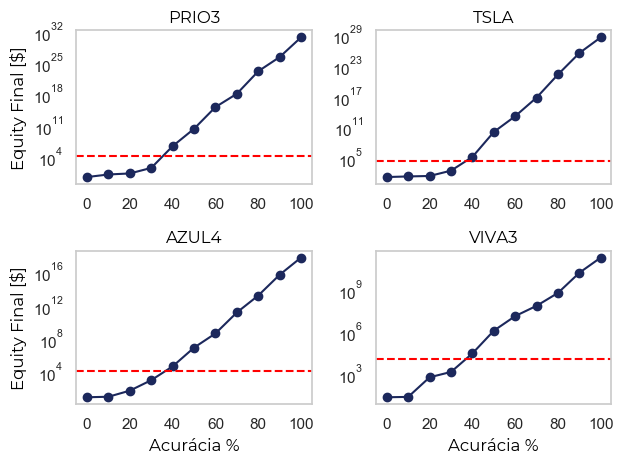
\includegraphics[width=1\linewidth]{imagens/equity_x_acur.png}
    \caption{Retorno por acurácia nos 4 ativos principais.}
    \label{fig:retorno-acuracia}
\end{figure}

Concluímos que um modelo com cerca de 40\% de acurácia é suficiente para lucrar consistentemente.

\subsubsection{Quantidade de dados de treinamento x Retorno}
Analisamos como a quantidade de dados de treinamento influencia o retorno obtido durante o período de backtest. Em cada modelo, consideramos os dados de treinamento começando em um ano específico até 2023 (sendo 2024 o ano de backtest). Variamos o ano inicial e calculamos os retornos.

Os gráficos abaixo mostram os retornos obtidos para cada ação, com a linha vermelha representando o montante inicial.

\begin{figure}[H]
    \centering
    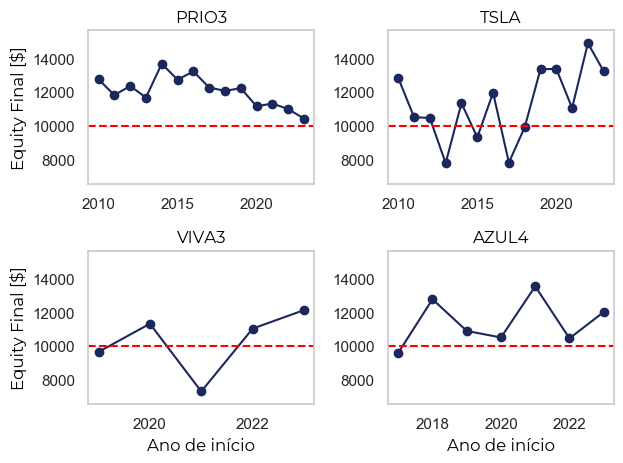
\includegraphics[width=1\linewidth]{imagens/equity_x_anoinic.png}
    \caption{Retorno em função do ano inicial de dados de treinamento.}
    \label{fig:retorno-anoinicial}
\end{figure}

Não foi identificada uma relação clara entre a quantidade de dados de treino e o desempenho do modelo.

\subsection{Quantidade de dados de treinamento x Win Rate}
Essa análise é semelhante à anterior, mas aqui investigamos a taxa de acerto (win rate) das transações do modelo.

Os gráficos abaixo mostram o win rate em função do ano inicial de treinamento para os 4 ativos analisados.

\begin{figure}[H]
    \centering
    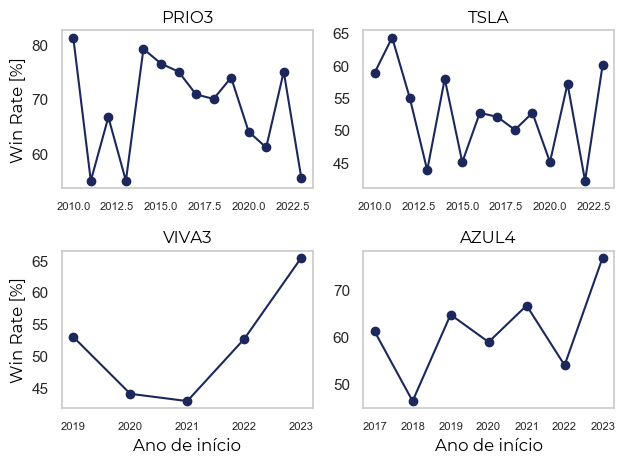
\includegraphics[width=1\linewidth]{imagens/win_x_rate_x_anoinicio.png}
    \caption{Taxa de acerto em função do ano inicial de dados de treinamento.}
    \label{fig:winrate-anoinicial}
\end{figure}

Novamente, não observamos uma relação evidente entre a quantidade de dados de treino e o desempenho do modelo.

\subsection{Análises dos resultados}

\subsubsection{Ações externas}
Para 20 ações com movimentação diária média e diferentes níveis de volatilidade (baseados em retorno logarítmico), testamos o modelo sem tunagem de hiperparâmetros. A seguir, apresentamos as análises realizadas:

\paragraph{Volatilidade x Acurácia}
A relação entre a volatilidade das ações e a acurácia obtida está representada no gráfico abaixo:

\begin{figure}[H]
    \centering
    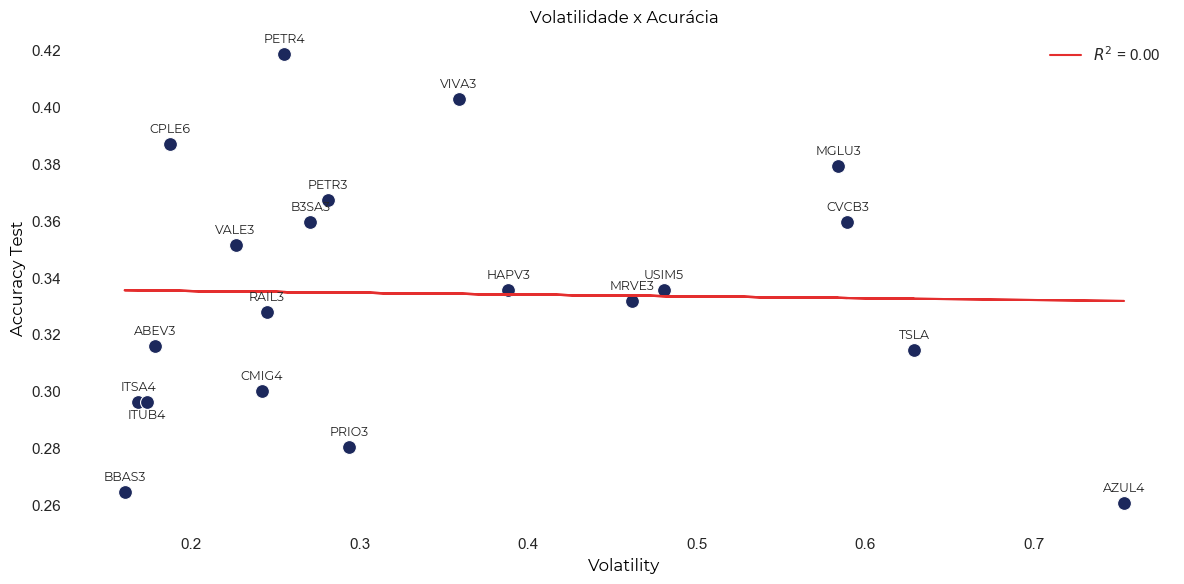
\includegraphics[width=1\linewidth]{imagens/vol_x_acur.png}
    \caption{Volatilidade x Acurácia.}
    \label{fig:volatilidade-acuracia}
\end{figure}

Não foi encontrada correlação significativa entre essas variáveis.

\paragraph{Volatilidade x Retorno percentual}
O gráfico a seguir mostra o retorno percentual em função da volatilidade.

\begin{figure}[H]
    \centering
    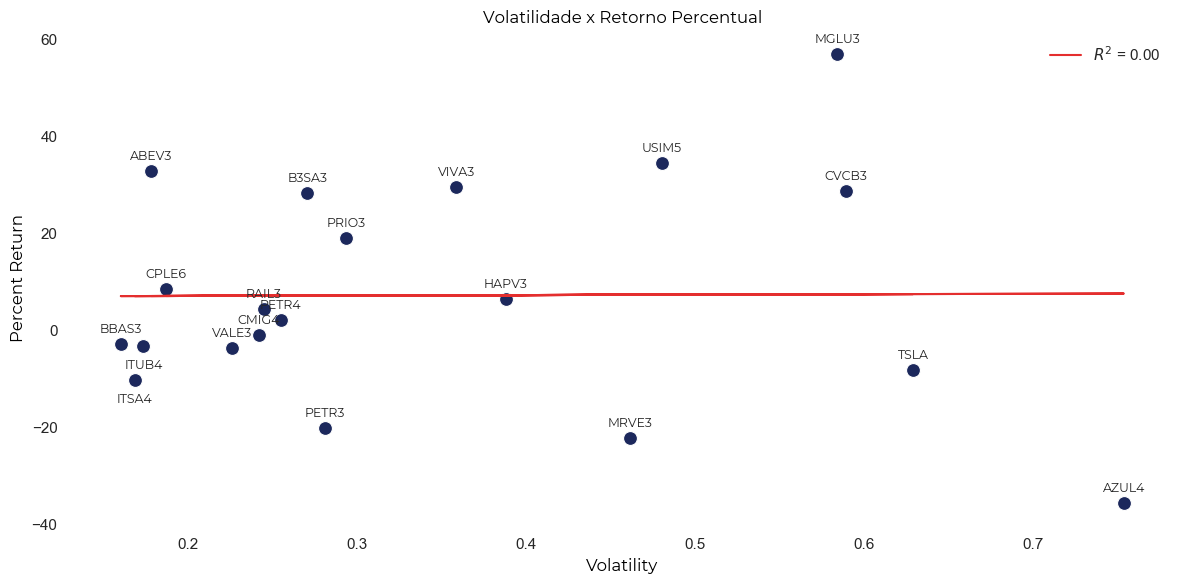
\includegraphics[width=1\linewidth]{imagens/vol_x_percentret.png}
    \caption{Volatilidade x Retorno percentual.}
    \label{fig:volatilidade-retorno}
\end{figure}

Mais uma vez, não observamos correlação entre essas variáveis.

\paragraph{Volatilidade x Win Rate}
Por fim, analisamos a relação entre a volatilidade e a taxa de acertos (win rate).

\begin{figure}[H]
    \centering
    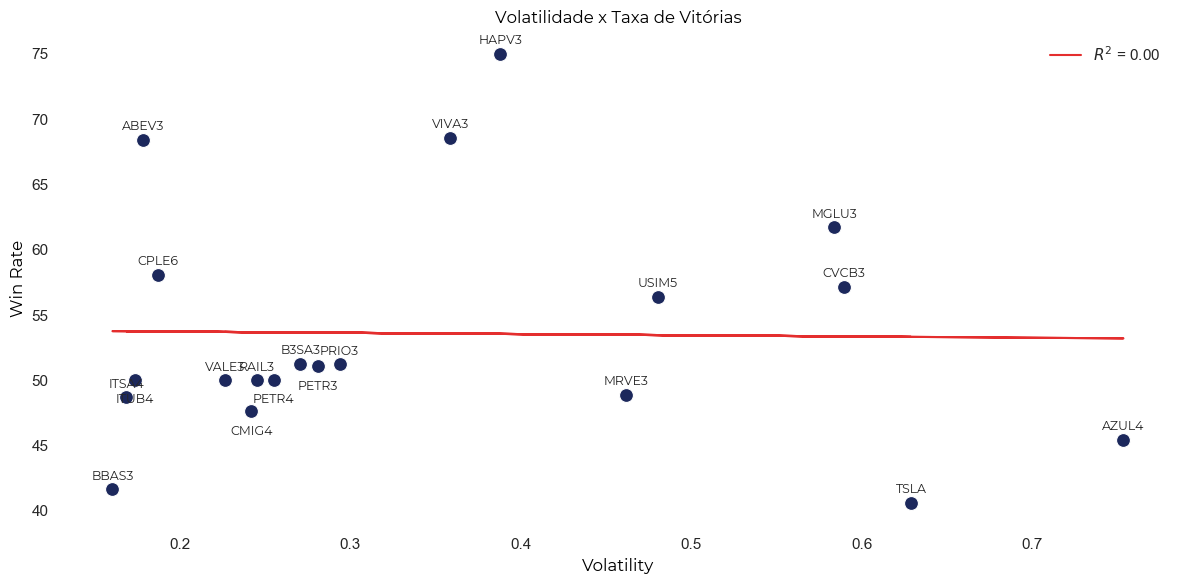
\includegraphics[width=1\linewidth]{imagens/vol_x_winrate.png}
    \caption{Volatilidade x Win Rate.}
    \label{fig:volatilidade-winrate}
\end{figure}

Não encontramos correlação significativa nessa análise também.

\subsubsection{Análise do número de features}
Realizamos análises para determinar como o número de indicadores utilizados influencia os resultados do modelo. O objetivo foi investigar a presença de overfitting e identificar um número ideal de features.

\paragraph{Número de indicadores x Retorno}
O gráfico abaixo mostra a relação entre o número de indicadores e o retorno obtido.

\begin{figure}[H]
    \centering
    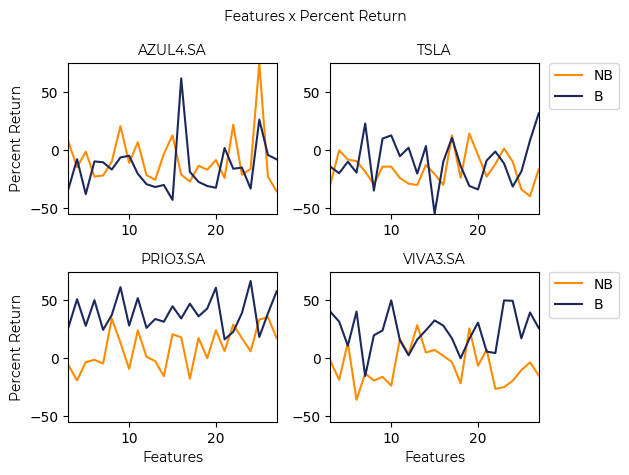
\includegraphics[width=1\linewidth]{imagens/features_x_percent_return.png}
    \caption{Número de indicadores x Retorno percentual.}
    \label{fig:features-retorno}
\end{figure}

Os dados binarizados apresentaram desempenho superior em alguns casos (notadamente PRIO3 e VIVA3), enquanto os dados não binarizados tiveram resultados mais inconsistentes.

\paragraph{Número de indicadores x Acurácia}
A seguir, analisamos como o número de indicadores influencia a acurácia do modelo.

\begin{figure}[H]
    \centering
    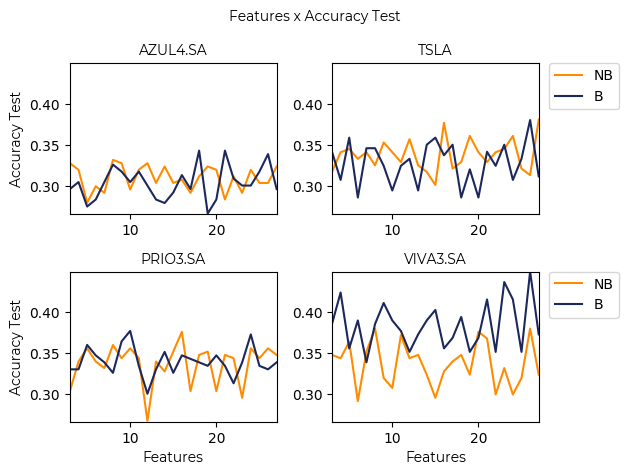
\includegraphics[width=1.0\linewidth]{imagens/features_x_accurtest.png}
    \caption{Número de indicadores x Acurácia.}
    \label{fig:features-acuracia}
\end{figure}

A única ação que alcançou cerca de 40\% de acurácia (o threshold definido anteriormente) foi VIVA3 com dados binarizados.

\paragraph{Features mais relevantes}
Por fim, identificamos as features mais relevantes para o modelo. Para isso, contamos quantas vezes cada indicador é utilizado no conjunto de dados, realizando a substituição dos nomes abreviados para os nomes completos dos indicadores. Além disso, o cálculo da frequência leva em consideração as janelas dos indicadores para ajustar a contagem, refletindo a quantidade de vezes que um indicador foi considerado relevante para a classificação. O gráfico a seguir destaca essas informações:

\begin{figure}[H]
    \centering
    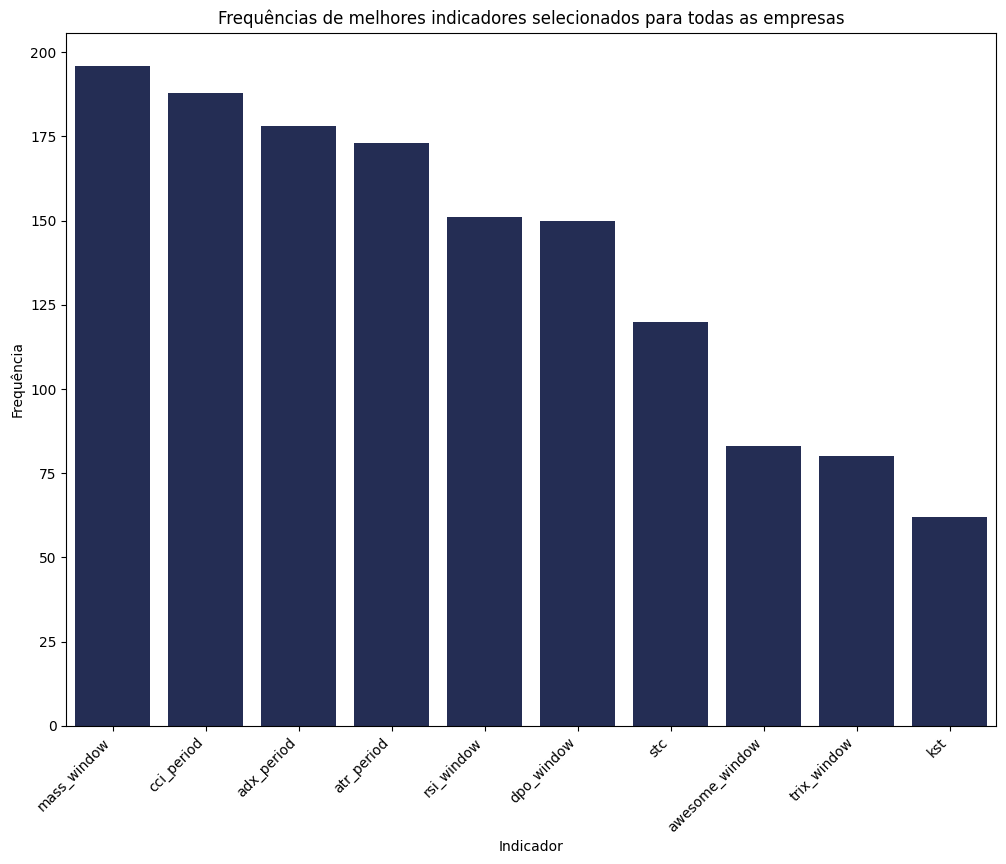
\includegraphics[width=1\linewidth]{imagens/features_importance.png}
    \caption{Importância das features no modelo.}
    \label{fig:features-importance}
\end{figure}

Notamos que os recursos que mais contribuíram para a importância foram, em ordem, o \texttt{Mass Index}, o \texttt{Commodity Channel Index} e o \texttt{Average Directional Index}, seguido pelo \texttt{Average True Range}. Isso indica que esses recursos têm alta importância para a maioria das variáveis.


\subsection{Melhores resultados}
Então, pegamos os melhores hiperparâmetros encontrados na validação e aplicamos o backtest com esses resultados. Obtivemos assim os seguinte resultados:

\begin{table}[h!]
\centering
\begin{tabular}{|c|c|c|}
\hline
\rowcolor{white!20} 
\textbf{}      & \textbf{Não binarizado} & \textbf{Binarizado} \\ \hline
\textbf{AZUL}  & \cellcolor{green!30}4\%  & \cellcolor{red!30}-32\% \\ \hline
\textbf{PRIO}  & \cellcolor{green!30}55\% & \cellcolor{green!30}26\% \\ \hline
\textbf{VIVA}  & \cellcolor{red!30}-30\% & \cellcolor{green!30}24\% \\ \hline
\textbf{TSLA}  & \cellcolor{green!30}17\% & \cellcolor{red!30}-4\%  \\ \hline
\end{tabular}
\caption{Tabela com valores binarizados e não binarizados.}
\end{table}

A análise mostra que, embora o modelo tenha alcançado bons desempenhos em alguns ativos, os resultados não foram consistentes para todos. Por exemplo, no caso de AZUL, o modelo binarizado apresentou uma queda significativa no desempenho, enquanto para PRIO e VIVA o mesmo modelo obteve resultados positivos.

Portanto, embora alguns cenários indiquem o potencial do modelo, não foi possível garantir a eficiência de forma geral devido à variação nos retornos entre diferentes ativos.

\newpage
\section{Possíveis Melhorias}

\begin{enumerate}
    \item \textbf{Melhor análise dos hiperparâmetros e do funcionamento do modelo Random Forest:}  
    Apesar do uso da Random Forest apresentar resultados satisfatórios, uma análise mais aprofundada dos indicadores que passamos para o modelo poderia ter elevado seu desempenho.

    \item \textbf{Utilização de uma variedade maior de modelos de machine learning:}  
    O trabalho se limitou à utilização do modelo Random Forest, mas o desempenho poderia ser comparado com outros algoritmos, como \textit{Gradient Boosting Machines} (e.g., XGBoost, LightGBM), \textit{Support Vector Machines} (SVM) e redes neurais. Isso poderia proporcionar uma melhor análise dos indicadores.

    \item \textbf{Melhor estudo dos indicadores:}  
    Os indicadores utilizados no modelo foram principalmente de \textit{trend following}, com valores fixos. Um estudo mais detalhado sobre a inclusão de outros tipos de indicadores, como osciladores (e.g., RSI, MACD) ou métricas de volatilidade, poderia agregar diversidade aos \textit{features} e, possivelmente, melhorar a capacidade preditiva do modelo.
\end{enumerate}

\newpage
\section{Conclusão}

Este trabalho apresentou uma abordagem para análise de mercado utilizando aprendizado de máquina, com foco no modelo Random Forest. Durante o processo, foi possível identificar os \textit{features} mais relevantes, o que contribuiu significativamente para a interpretação e melhoria do modelo. Entre os principais resultados, destaca-se:

\begin{itemize}
    \item A definição de um \textit{threshold} de 40\%, que se mostrou eficaz como critério de decisão para operar no mercado.
    \item A identificação de variáveis importantes que impactam diretamente o desempenho do modelo.
    \item A validação de que, sob as condições analisadas, o modelo foi capaz de gerar lucros na maioria do tempo.
\end{itemize}

O trabalho demonstrou o potencial do aprendizado de máquina para tomada de decisão em mercados financeiros, abrindo espaço para futuras melhorias e estudos mais aprofundados.

\newpage
\printbibliography %Printa bibliografia
\end{document}